

\section{Introduction}

Synthetic data has emerged as a key technique for building large language models due to its cost-effectiveness and scalability~\citep{dubey2024llama3herdmodels, nvidia2024nemotron4340btechnicalreport, deepseekai2024deepseekv2strongeconomicalefficient}. 
In particular, synthetic data is well suited for mathematical reasoning where the performance improvements with synthetic data scaling are yet to saturate~\citep{zeng2024skyworkmathdatascalinglaws, chan2024scalingsyntheticdatacreation, yang2024qwen25mathtechnicalreportmathematical}. 
However, access to this progress is limited because the current largest math datasets remain \emph{closed-source}~\citep{zeng2024skyworkmathdatascalinglaws, yang2024qwen25mathtechnicalreportmathematical}. 
The closed nature of these datasets introduces two major issues. First, concerns over data leakage erode trust in reported benchmark results~\citep{aiyappa-etal-2023-trust}. E.g., \citet{zhang2024carefulexaminationlargelanguage} show a drop of more than 10\% for popular LLMs on an unpublished test set which is distributionally similar to the popular grade school math benchmark GSM8K~\citep{cobbe2021gsm8k}. Second, it prevents practitioners from fully understanding the impact of data composition and algorithmic choices~\citep{azerbayev2024llemma, soldaini-etal-2024-dolma}. 



Among open-source alternatives, the recent NuminaMath dataset \citep{li2024numinamath} has the largest collection of questions collected from diverse sources. However, its restrictive license—likely due to the use of GPT-4o in data processing and synthesis—limits its broader use.
Similarly, other popular math instruction tuning datasets, such as MetaMathQA~\citep{yu2024metamath} and MathInstruct~\citep{yue2024mammoth}, have also utilized GPT models for data synthesis, which prohibits their usage in non-commercial settings.  
A notable exception is the OpenMathInstruct-1~\citep{toshniwal2024openmathinstruct} dataset, one of the biggest open-source math reasoning datasets, where solutions are synthesized using open-weight models. 
However, OpenMathInstruct-1 has two key limitations. Firstly, its question diversity is limited, since all the questions in the dataset are drawn from the training sets of MATH~\citep{hendrycks2021measuringmathematicalproblemsolving} and GSM8K~\citep{cobbe2021gsm8k}. 
Secondly, at the time of its release, there was a sizable gap in the math reasoning capabilities of open and closed-source models. As a result, the dataset underrepresents more challenging problems compared to its GPT-based counterparts~\citep{gou2024toratoolintegratedreasoningagent}. 


The recent emergence of \emph{frontier} open-weight models~\citep{dubey2024llama3herdmodels, deepseekai2024deepseekv2strongeconomicalefficient} has made it possible to create high-quality, commercially permissible math reasoning datasets. 
In this paper, we use the recently released Llama3.1 family of models to generate synthetic math instruction tuning (SFT) data, and evaluate the quality of the math reasoning data by finetuning the smaller 8B and 70B base models.\footnote{
Data and models are available at \url{https://huggingface.co/collections/nvidia/openmath-2-66fb142317d86400783d2c7b}\\
Code is available at \url{https://github.com/Kipok/NeMo-Skills}}   
To create OpenMathInstruct-2, we conduct careful ablation studies using the MATH dataset to determine design choices that impact the final SFT performance. The highlights of our findings include:
\begin{itemize}
    \item  \emph{Chain-of-Thought (CoT) Solution Format}: Excessive verbosity can be detrimental to the SFT performance. Our proposed CoT format outperforms Llama's CoT format by 3.9\% while being 40\% shorter in solution length. Using \emph{base model template} (Figure~\ref{fig:base_prompt} in Appendix) significantly increases the ability of instruct models to follow few-shot examples of our proposed format.
    \item \emph{Choice of Data Generation Model}: 
    Controlling for the size of the SFT data, the performance on data generated by a strong teacher model surpasses that of data produced by a weaker student model by 7.8\%.
    \item \emph{Robustness of SFT}: 
    With both removing low-quality solutions and introducing them by design, we find SFT performance to be robust to the presence of up-to 20\% low-quality data. 
    \item \emph{Impact of Question Diversity}: 
    Controlling for SFT data size, we find that question diversity has a huge positive impact on SFT performance. Increasing the number of unique questions from 1K to 6.5K leads to 10.5\% improvement on MATH validation set.
\end{itemize}



\begin{figure*}[t]
    \centering
    \begin{minipage}[t]{0.48\linewidth}
        \centering
        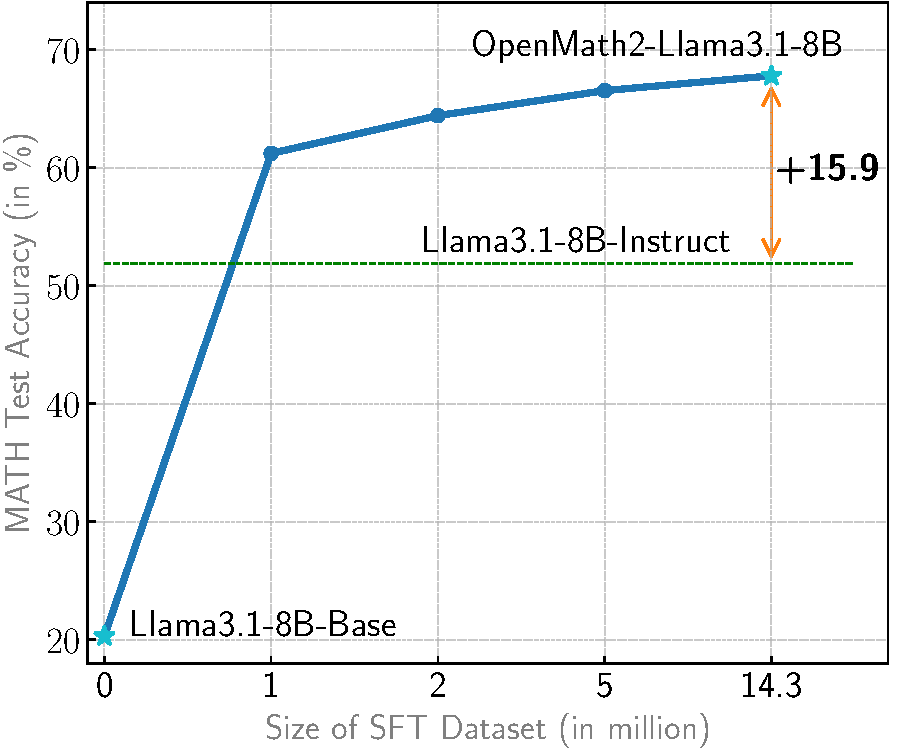
\includegraphics[width=\linewidth]{plots/scaling_plot.pdf}
        \caption{Performance of \texttt{Llama3.1-8B-Base} on MATH after finetuning on increasing proportions of OpenMathInstruct-2.}
        \label{fig:sft_scale}
    \end{minipage}
    \hfill
    \begin{minipage}[t]{0.48\linewidth}
        \centering
        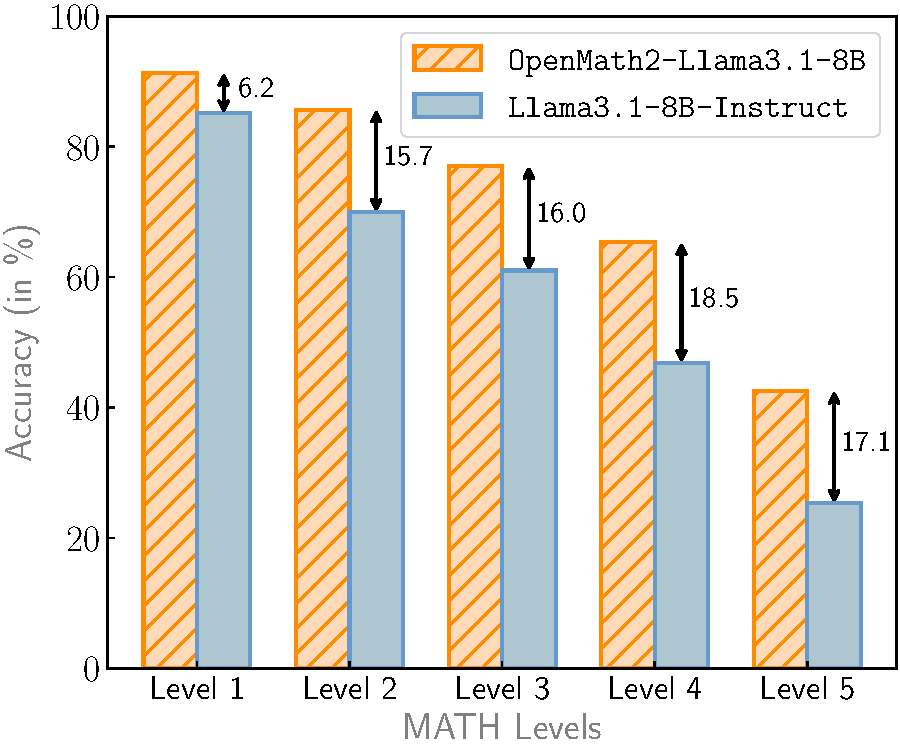
\includegraphics[width=\linewidth]{plots/math_level_comp.pdf}
        \caption{Comparison of \texttt{OpenMath2-Llama3.1-8B}  and \texttt{Llama3.1-8B-Instruct} on accuracy across MATH difficulty levels.}
        \label{fig:math_level_comp}
    \end{minipage}
% \vspace{-0.15in}
\end{figure*}



Based on the above findings, we create \dataset with data synthesized using \texttt{Llama-3.1-405B-Instruct}. 
To construct this dataset we prompt an LLM to (a) synthesize solutions to the original MATH and GSM8K training set questions and (b) create new question-solution pairs similar to the training set questions.   
To ensure there is no test set contamination among the synthesized questions, we perform thorough decontamination using the \texttt{lm-sys} pipeline  \citep{yang2023rethinkingbenchmarkcontaminationlanguage}, followed by manual inspection (Section~\ref{sec:llm_decontamination}). 
Figure~\ref{fig:data_overview} provides an overview of the entire dataset construction pipeline. 
The final dataset consists of \datasize question-solution pairs with \uniqquesns unique questions, including 592K synthesized questions. Thus, \dataset is about 8 times bigger than the previous biggest standalone open-source dataset~\citep{toshniwal2024openmathinstruct}. 

The high-quality of \dataset is illustrated by the strong performance of the finetuned models. The \texttt{OpenMath2-Llama3.1-8B model}, which is the \texttt{Llama3.1-8B-Base} model finetuned with \dataset, outperforms \texttt{Llama3.1-8B-Instruct} by an absolute 15.9\% on MATH with just SFT (see Figure~\ref{fig:sft_scale} and \ref{fig:math_level_comp}). 
With a performance of 67.8\% on MATH, \texttt{OpenMath2-Llama3.1-8B} is one of the strongest sub-10B open-source models.\footnote{We refer to open-weight base models instruction tuned with publicly released data as open-source.}  
Our best-performing model, \texttt{OpenMath2-Llama3.1-70B}, has an accuracy of 71.9\% on MATH which outperforms \texttt{Llama3.1-70B-Instruct} by 3.9\%.
To support the open-source efforts, we will release all our fine-tuned models, code, and the \dataset dataset.  
\begin{figure*}
    \centering
    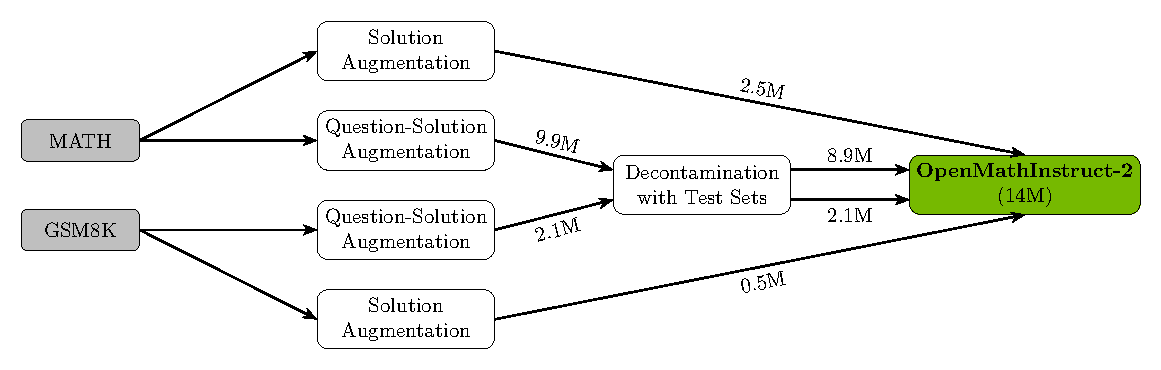
\includegraphics[width=\linewidth]{figures/data_diagram.pdf}
    \caption{Overview of the data generation pipeline used for \dataset.}
    \label{fig:data_overview}
\end{figure*}

